\Lecture{Jayalal Sarma}{Aug 31, 2015}{16}{On Transitive Group Actions and their properties}{Mitali Bafna}{$\gamma$}{K Dinesh}

In the last lecture, we saw algorithms for solving coloured $\gi$ when the
colour class are bounded size. In this lecture, we will see some new concepts 
for computing $Aut(X)$ for graph $X$ which has more a divide and conquer
flavour.

\section{Transitive Group action and Blocks}
We start with the following example. Consider a complete binary tree $T$ of 
depth $k$. Let us ask : how does $Aut(X)$ act on the leaves of $T$. If we
consider the action of $Aut(X)$ on set the leaves of $T$, then we can
observe that there is an automorphism that maps any leaf to any other leaf.
For example, the permutation which takes $1$ to $3$ and $2$ to $4$ and fixes
the rest takes leaf $1$ to leaf $3$.
\begin{figure}[htp!]
	\centering
	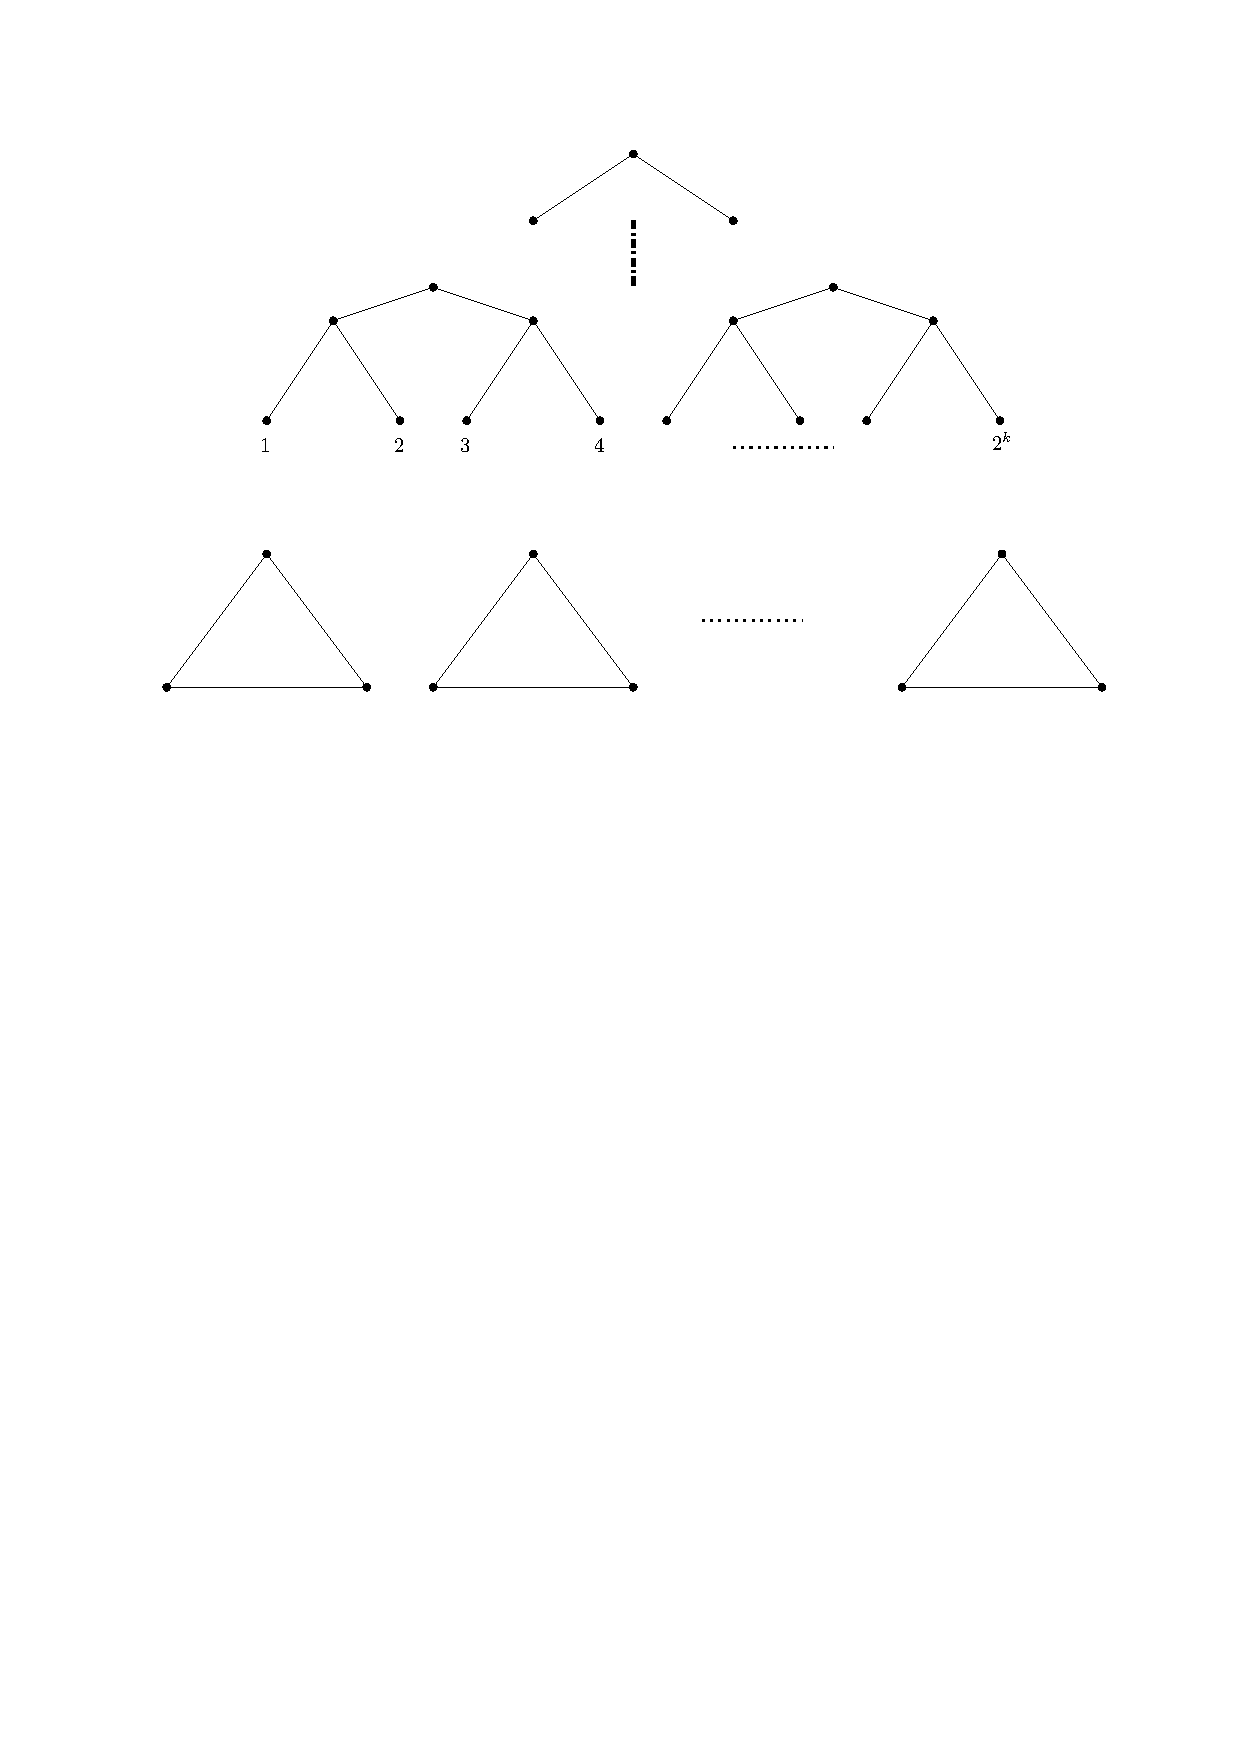
\includegraphics[scale=0.68]{images/transitive}
	\caption{Transitive group action}
	\label{fig:transitive}
\end{figure}

This property of the group action is called Transitive.
\begin{definition}[Transitive Group Action]
	For a group $G \le S_n$ acting on a set $\Omega$, the action is said
	to be transitive if, for all $\alpha, \beta \in \Omega$, there exists
	a $g \in G$ such that $\alpha^g = \beta$.
\end{definition}
In the above example, we can see $Aut(X)$ acts transitively on the set of
leaves of $T$.

Observe that any nontrivial automorphism can either map $1$ and $2$ among
each other (i,e. $1$ to $2$ and $2$ to $1$) or map both $1$ and $2$ to say
$3$ and $4$. But it can never map say $1$ to $2$ and $2$ to $3$ as it violate
adjacency. Hence the leaves with common ancestors always gets moved in a pair.

Consider another graph $X$ which is $k$ vertex disjoint triangles. Consider
the action of $Aut(X)$ on $V(X)$. We again observe a similar phenomena as
before. There is an automorphism that takes any vertex to any vertex. Also
any automorphism maps vertices in a triangle to itself or to a totally 
different triangle. Hence either a triangle is mapped to itself or is moved
whole together as a block.

These two examples motivate the notion of blocks.

\begin{definition}[Blocks]
	For a group $G$ acting on $\Omega$, a set $\Delta \subseteq \Omega$ 
	is a block if $\forall g \in G, \Delta^g = \Delta$ or 
	$\Delta^g \cap \Delta = \phi$.
\end{definition}
We observe that $\Omega$ and the singletons sets $\{\alpha\}$
where $\alpha \in \Delta$ form blocks trivially. 

Apart from the fact that such block structure naturally arise in the action
in many graphs, they also can be potentially used to compute $Aut(X)$. In the
case of trees, we can start with trivial blocks whose automorphisms are also
trivial, combine the blocks and obtain the automorphism for larger blocks and
proceed in a bottom up manner building larger blocks and thereby get the
automorphism of the entire tree.
%\footnote{This is not a rigorous argument and
%is more of an idea to use blocks for computing automorphism.}.

\section{Primitive actions}
We saw that for $\Omega = [n]$ and $G = S_n$, the sets $\Omega$, $\{1\}, \{2\},
\ldots, \{n\}$ does form blocks. Are there any other blocks ? The answer is
no since for any $T \subsetneq \Omega$ of size at least $2$, there is a
permutation in $G$ that fixes one and moves the other. Hence these are the only
blocks and we call such blocks trivial blocks and the action as
\emph{primitive}.

\begin{definition}[Primitive action]
	A group action of $G$ on $\Omega$ is primitive if there are no
	non-trivial blocks. An action which is not primitive is called
	imprimitive.
\end{definition}

Let us consider another action where $G \subseteq S_n$ acts on itself via
right multiplication (see Lecture 8). That is for $g' \in G$, the action
takes $g$ to $gg'$ with $\Omega = G$. This action is clearly transitive as
given any $g,h \in G$, $g' = g^{-1}h$ takes $g$ to $h$. Also, if $G$ has a 
non-trivial \footnote{That is $H$ is not $G$ or $\{id\}$} subgroup $H$ then
the action is not primitive.  This is because, the cosets of $H$ in $G$ form 
the non-trivial blocks. That is, for any two shift of $H$ say $Hg_1, Hg_2$,
either $Hg_1 = Hg_2$ or $Hg_1 \cap Hg_2 = \emptyset$ (Lemma~\ref{lag1}) which
we observed in the proof of Lagrange's theorem.

This shows that if $G$ has a non-trivial subgroup, then the action is not
primitive. Is the converse observation that $G$ has only trivial
subgroup imply the action is primitive also true ? We will see in the next 
lecture that the converse holds too. This gives a very interesting
characterization or a ``connection'' between blocks which are combinatorial in
nature and subgroups which are algebraic in nature.

We first show that action of $G$ on $\Omega$ induces a partition to form a
block system.

\begin{definition}[Block System]
A partition of $\Omega$ into sets such that each part is a block under the action of G.
\end{definition}

To see this, we will explore some properties of blocks.
\begin{claim}
	Let $G \le S_n$ be a group acting on $\Omega$ and $\Delta \subseteq \Omega$
	be a block. 
	Then for any $g \in G$, the
	following holds.
	\begin{enumerate}
		\item  $\Delta^g$ is also a block
		\item  $|\Delta^g|  = |\Delta|$
	\end{enumerate} \label{cl:block-prop}
\end{claim}
\begin{proof}
	\begin{description}
		\item[Proof of 1] We give a proof by contradiction. Suppose
			there exists a $g \in G$ for which $\Delta^g$ is not a
			block. By definition, since $\Delta^g$ is not a
			block, there exists an $h \in G$ such that 
			\[ \Delta^{gh} \ne \Delta^g \text{ and } 
			\Delta^{gh} \cap \Delta^g \ne \emptyset\]
			Hence there exists $\beta \in \Delta^g$ but $\beta^h
			\not \in \Delta^g$ and there is a $\gamma \in
			\Delta^{gh} \cap \Delta^g$.
			Since $\beta \in \Delta^g$, there exists an $\alpha
			\in \Delta$ such that $\alpha^{gh} \not \in
			\Delta^g$. Hence $\alpha^{ghg^{-1}} \not \in \Delta$
			while $\alpha^{ghg^{-1}} \in \Delta^{ghg^{-1}}$. Hence
			$\Delta \ne \Delta^{ghg^{-1}}$. 

			Since $\gamma \in \Delta^g$ and $\gamma \in
			\Delta^{gh}$, there exists an $\omega,\delta \in 
			\Delta$ such that $\gamma = \omega^g = \delta^{gh}$. 
			Hence $\omega =	\gamma^{ghg^{-1}} \in 
			\Delta^{ghg^{-1}}$. Along with the fact that
			$\omega \in \Delta$, we get that $\Delta \cap
			\Delta^{ghg^{-1}}\ne \emptyset$. But $\Delta \ne
			\Delta^{ghg^{-1}}$ and $\Delta \cap
			\Delta^{ghg^{-1}}\ne \emptyset$ contradicts the fact
			that $\Delta$ is a block. Hence it must be that
			$\Delta^g$ is also a block.
		\item[Proof of 2] 
		This follows from the fact that $g \in G$ is a permutation
		and it is a bijection map.
	\end{description}
\end{proof}

If the group action is transitive, then $\Omega$ is partitioned by the
blocks.
\begin{claim} For a group $G \le S_n$ that acts transitively on $\Omega$ with
	$\Delta \subseteq \Omega$ as a block, the following holds.
	\begin{enumerate}
		\item $\bigcup_{g \in G} \Delta^g = \Omega$
		\item For any $g_1, g_2 \in G$,  $\Delta^{g_1} \cap
			\Delta^{g_2} \ne \phi \Rightarrow \Delta^{g_1} =
			\Delta^{g_2}$.  
		\item $|\Delta|$ must divide $|\Omega|$.
	\end{enumerate}
\end{claim}
\begin{proof}
	\begin{description}
		\item[Proof of 1] 
Let $k \in \Delta$. For any $k' \in \Omega$, since the action is transitive
$\exists g$ such that  $k^g = k'$ giving $k' \in \Delta^g$. Hence $\Omega
\subseteq \bigcup_{g \in G} \Delta^g $. The other containment is direct and
hence they are equal.
		\item[Proof of 2]
		This is true since, with $\Delta^{g_1}$ being a block
		(Claim~\ref{cl:block-prop}(1)), either $\Delta^{g_1} =
		\Delta^{g_1(g_1^{-1}g_2)}$ or  $\Delta^{g_1} \cap
		\Delta^{g_1(g_1^{-1}g_2)} = \emptyset$.
	\item[Proof of 3] The above two claims prove that $\Omega$ is partitioned
		into subsets with equal cardinality and all of them have the
		same size as $|\Delta|$ (Claim~\ref{cl:block-prop}(2)). So
		$|\Delta|$ must divide $|\Omega|$.  \end{description}
\end{proof}

We get an immediate sufficient condition on $\Omega$ for the action of any 
$G$ to be primitive. 
\begin{corollary}
	If $|\Omega |$ is prime, then the action of any $G \le S_n$ on
	$\Omega$ is bound to be primitive.  
\end{corollary}

Before ending, let us see why transitive actions are important. For a general
group $G$ whose action is not necessarily transitive, if we look at the
action on elements of an orbit, the action becomes transitive. Hence we can
use our divide and conquer strategy to build blocks and at least obtain
automorphism group for the orbits.
%\dsay{I am not very clear about this para}

\Lecture{Jayalal Sarma}{Sep 1 2015}{17}{Characterisation of
Primitivity}{Mitali Bafna}{$\gamma$}{K Dinesh}

In the last lecture, we saw transitive and primitive group action. In this
lecture, we give an algebraic characterization of primitive group actions.

We need the notion of maximal subgroup of a group.
\begin{definition}[Maximal Subgroup]
$H \leq G$ is a maximal subgroup if there does not exist an $H'$ such that 
$H \lneq H' \lneq G$ where $\lneq$ denotes strict subgroup containment.
\end{definition}

The main theorem is the following.
\begin{theorem}
	Suppose $G \le S_n$ acts transitively on $\Omega$. Then the action is
	primitive if and only if $\exists \alpha \in \Omega$ such that
	$G_{\alpha}$ is the maximal subgroup of $G$ where $G_\alpha$ is the
	stabilizer of $\alpha$
	\label{thm:primitive-action}
\end{theorem}

Recall the action (in the last lecture) for $G \le S_n$ where $G$ acts on
itself. We saw that if $G$ has any non-trivial subgroup $H'$, the action is
not primitive. If $H'$ has a super group $H$ then, there is a nice relation
between the cosets induced by $H$ and $H'$ on $G$ described as an exercise
below.
\begin{exercise}
%{subgroup-cost-structure}
	Let $H' \lneq H \lneq G$. The cosets induced by $H$ and $H'$
	partitions $G$. Show that the partition induced by $H'$ is a
	refinement of the partition induced by $G$. That is, show that
	every cosets of $H'$ in $G$ must be contained in some coset of $H$ in
$G$.  
\end{exercise}

\begin{figure}[htp!]
	\centering
	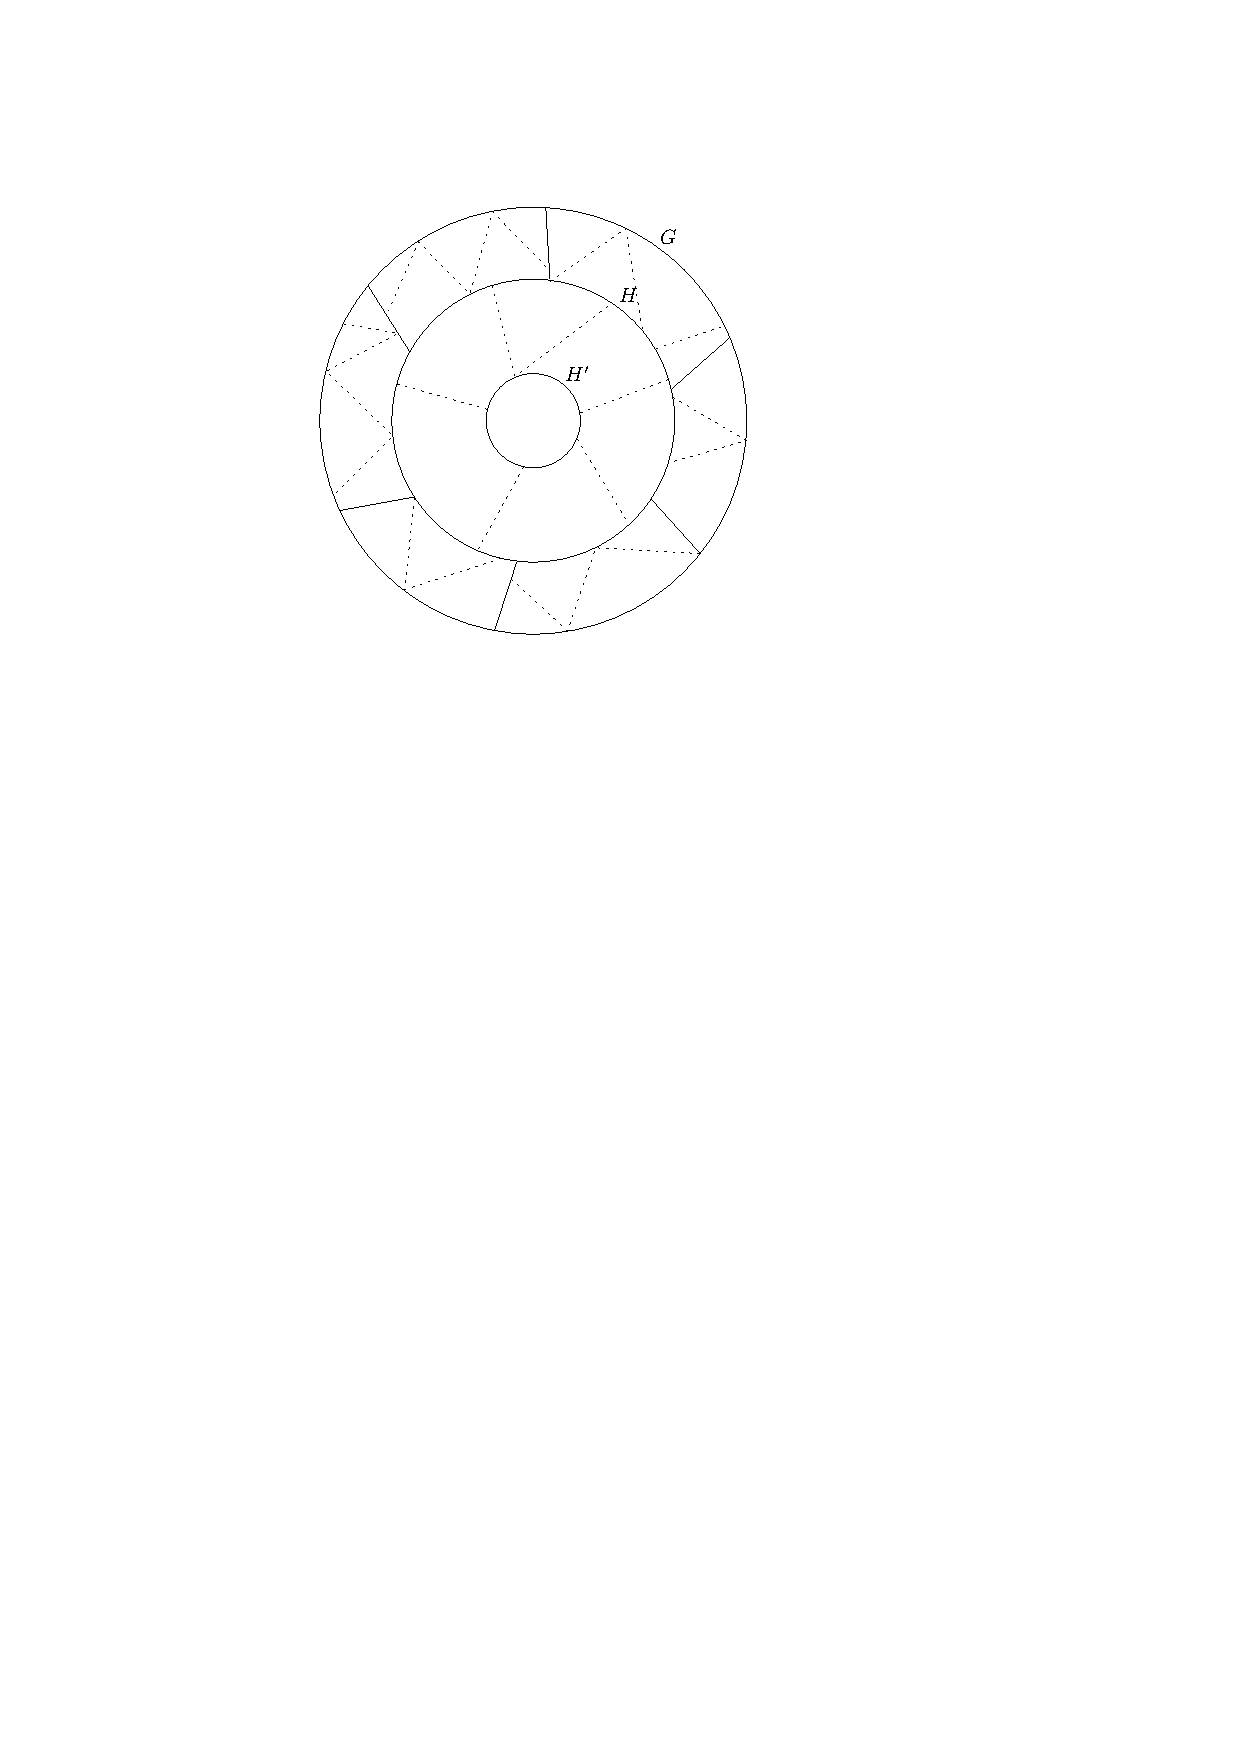
\includegraphics[scale=0.7]{images/coset}
	\caption{Coset structure of subgroups $H$ and $H'$. Dotted ones are
	cosets of $H'$.}
	\label{fig:coset}
\end{figure}

With this structure in place, we can also consider the cosets of $H'$ 
as the elements and consider the action of $G$ on this set. Since $H$ has a
smaller subgroup $H'$, there are non-trivial blocks for this action. The
action moves all those cosets of $H'$ that fall in a coset of $H$. This must
happen as this is precisely the action of $G$ on the cosets of $H$.
Hence the collection of cosets of $H'$ within a cost of $H$ forms a block.
The characterization theorem for primitive action tells that if $H'$ does not
have a larger subgroup $H$, then the action is bound to be primitive. We state
this as a corollary.

\begin{corollary}
	For $H' \lneq G$ and $H'$ does not have a super group $H$ in $G$, the
	action of $G$ on the cosets of $H'$ in $G$ must be primitive.
\end{corollary}

Before going to the proof, we first show that the following variant of 
Theorem~\ref{thm:primitive-action} where $\exists \alpha$ is replaced by 
$\forall \alpha$ is also true. For this, it suffices to prove the following
claim.

\begin{claim}
	For a group $G$ acting transitively on $\Omega$, if there exists an
	$\alpha \in \Omega$ such that $G_\alpha$ is maximal subgroup of $G$,
	then for all $\beta \in \Omega$, $G_\beta$ is also maximal subgroup of
	$G$.
	\label{cl:prop-trans}
\end{claim}
\begin{proof}
	Suppose there exists $\alpha$ such that $G_\alpha$ is maximal subgroup
	of $G$. Since $G$ is transitive, for any $\beta \in \Omega$, there
	exist a $g$ such that $\alpha^g = \beta$. Note that $G_\alpha$ and
	$G_\beta$ can be related as $g^{-1}G_\alpha g =
	G_\beta$. This is because,
	\begin{align*}
		G_\beta  =&  \{ g' ~|~ \beta^{g'} = \beta \} \\
			= & \{ g' ~|~ \alpha^{gg'} = \alpha^g \} \\
			= & \{ g' ~|~ \alpha^{gg'g^{-1}} = \alpha \} \\
			= & \{ g^{-1} hg ~|~ \alpha^{h} = \alpha \} &&
			[\text{Renaming $gg'g^{-1}$ as $h$}] \\
			= & g^{-1}G_\alpha g
	\end{align*}
	Now if $G_\beta$ has a larger subgroup containing
	it in $G$, then we can give a larger
	subgroup for $G_\alpha$ also which contradicts maximality\footnote{ If
		there is an $H'$ such that $G_\beta \lneq H' \lneq G$ then
		consider $g^{-1}H'g$ as it satisfy $G_\alpha \lneq g^{-1}H'g
	\lneq G$.}. 
\end{proof}
The pair of groups $G_\alpha$, $G_\beta$ in the previous claim are sometimes
called as conjugate pairs.
\begin{definition}[Conjugates]
	Subgroups $H,H'$ of a group $G$ are said to be conjugates, if there 
	exists a $g \in G$ such that $gHg^{-1} =H'$.
\end{definition}

\section{Proof of characterization}
We restate the characterization in the light of Claim~\ref{cl:prop-trans}.
\begin{theorem}
	Suppose $G \le S_n$ acts transitively on $\Omega$. Then the action is
	primitive if and only if $\forall \alpha \in \Omega$ such that
	$G_{\alpha}$ is the maximal subgroup of $G$ where $G_\alpha$ is the
	stabilizer of $\alpha$
	\label{thm:primitive-action-strong}
\end{theorem}
Note that both these theorems are equivalent. We now give a proof.

\begin{proof}[Proof of Theorem~\ref{thm:primitive-action-strong}]

The backward direction ($\Longleftarrow$): if $\forall \alpha \in G$,
$G_\alpha$ is maximal the maximal subgroup of $G$, then the action is
primitive.

We will prove the contrapositive that is, suppose that the action is not 
primitive then $\exists \alpha \in G$ such that , $G_\alpha$ is not a maximal 
subgroup.

Suppose $G$ does not act primitively on $\Omega$. Then there must be
non-trivial block $\Delta$ and $\alpha \in \Omega$ such that $\{\alpha\}
\subsetneq \Delta \subsetneq \Omega$. We need to show that there exists an $H$
such that $G_\alpha \lneq H \lneq G$. We show this in two steps.

\begin{description}
	\item [Show that $G_\alpha \le H \le G$ :]
Consider $H = \setstab(\Delta) = \{g \in
G ~|~ \Delta^g =\Delta \}$. We now show that $G_\alpha$ is a subgroup of $H$.
To show this, let $g \in G_\alpha$. Hence $\alpha^g = \alpha$ and $\alpha$ is
a common element in $\Delta$ and $\Delta^g$. Along with the fact that $\Delta$
is a block, we get that $\Delta = \Delta^g$. Hence $g$ fixes $\Delta$ which
gives that $g \in H$.  Hence $G_\alpha \leq H$. By definition of $H$, we have $H \le G$.
	\item [Both containments are strict :]
Let $\beta \neq \alpha$ belongs to $\Delta$. Such a $\beta$ must exist as
$\{\alpha\} \subsetneq \Delta$. Since $G$ is transitive, there exists a  $g
\in G$ such that $\alpha^g = \beta$.  Clearly 
$g \notin G_\alpha$. Now since $\beta \in \Delta \cap \Delta^g$ and $\Delta$
is a block, we get $\Delta^g = \Delta$ and $g \in H$.
\end{description}
Hence $G_\alpha \lneq H \lneq G$ and $G_\alpha$ is not maximal.

The forward direction ($\Longrightarrow$):
We again prove the contrapositive : if $\exists \alpha \in \Omega$ such that 
$G_\alpha$ is not a maximal subgroup, then the action is not primitive (i,e.
come up with a non-trivial block).

Suppose $\alpha \in \Omega$ be such that $G_\alpha \lneq H \lneq G$.  We will
produce a $\Delta$ such that $\Delta$ is a non-trivial block. We define 
$\Delta = \alpha^H$. Now we are left to show that the $\Delta$ chosen is
indeed a non-trivial block. To prove this, we need to show the following:
\begin{description}
	\item[$\{\alpha\} \subsetneq \Delta$ :] 
		From the Orbit-Stabiliser lemma (Lemma~\ref{lem:os}), we have
		that each coset of $G_\alpha$ in $G$ corresponds to a
		different element in the orbit of $\alpha$.  That is all the
		elements in a coset take $\alpha$ to the same element and if
		two cosets are different then their action on $\alpha$ is too.
		Mathematically, for $g_1,g_2 \in G$, 
		$g_1G_\alpha = g_2G_\alpha \Leftrightarrow
		\alpha^{g_1} = \alpha^{g_2}$.

	Since $G_\alpha \lneq H,\exists$ a coset $C \neq G_\alpha \in H$. Let
	$C = G_\alpha h$ where $h \in H$ is the coset representative.
	Now, $G_\alpha \neq C \Rightarrow \alpha  \ne
	\alpha^h = \beta$ for some $\beta \in \Omega$. But $\beta = \alpha^h
	\in \alpha^H = \Delta$.  So we have that $\{\alpha\} \subsetneq
	\Delta$.
	% proof done in class:
	%	Since $G_\alpha \lneq H$,
	%	there exists $g \in H$ such that $ g\not \in G_\alpha$. Hence
	%	$\alpha^g = \beta$ where $\beta \ne \alpha$. Also $\beta \in
	%	\Delta$ as $\beta$ is in the orbit of $g$. Hence $\{\alpha
	%	\} \subsetneq \{\alpha, \beta\} \subseteq \Delta$.

	\item[$\Delta \subsetneq \Omega$ :] 
	Since $H \lneq G$ and $G_\alpha \lneq H, \exists$ a coset $C$ of
	$G_\alpha$ in $G$ which does not belong to $H$. Let $g \in G$ be its
	coset representative. Since different cosets
	take $\alpha$ to different elements $\alpha^g \notin \alpha^H$. So we
	have that $\Delta = \alpha^H \subsetneq \alpha^G = \Omega$. 

	\item[$\Delta$ is a block :]
		We show that for any $g \in G$, either $\Delta^g = \Delta$ or
		$\Delta^g \cap \Delta = \emptyset$. Suppose $\Delta^g \cap
		\Delta = \emptyset$, we are done. Suppose $\Delta^g \cap
		\Delta \neq \emptyset$. We then show that $\Delta^g = \Delta$.
		
		Recall that $\Delta = \alpha^H$. Since $\Delta^g \cap \Delta
		\ne \emptyset$, 
		\begin{align*}
		& \exists h',h \in H, \alpha^{h'g} = \alpha^h \\ 
		\implies & h'gh^{-1} \in G_\alpha \\
		\implies & g \in H && [\text{Using $G_\alpha$ is a subgroup of
		$H$}] \\
		\implies & \Delta^g = \alpha^{Hg} = \alpha^H = \Delta
		\end{align*}
\end{description}
This completes the proof.
\end{proof}





